\chapter{Background}
\label{chapter:literature}

This chapter describes the background knowledge related to this thesis. The main focus is on software maintenance and knowledge sharing in agile organizations, but also
software process improvement guidelines and frameworks are presented to support change process in the case company. As measuring the change is important in software
process improvement, also the most relevant software maintenance metrics are described. Finally to solve the challenges, a set of common solutions is presented,
forming a basis of solution proposals applied to the case company's context. The time period of the articles reviewed was typically
last ten years for industry specific topics and last 20 years for more general topics.

\section{Software maintenance}

Software maintenance generally includes all of the activities that are done after the software has been delivered \citep{Sommerville2011}.
In modern agile frameworks the transition from
active development to maintenance phase might not be as clear cut as presented in the waterfall model, but it can be set to the first successful production deployment
that actually provides some business value.
Of course there might be new releases requiring active development, but the first version still stays in use in parallel and most likely needs some maintenance
every now and then. The maintenance phase is usually the longest phase for any software project as it might last for decades before the system
is eventually replaced with a newer one.
Taking the long lifespan into account, it is important to consider the maintainability of a system under development
as investing more time and money on improving maintainability in the early phase
could result in large savings in the future \citep{Sommerville2011}.

\subsection{Maintenance task types}

Software maintenance activities can be divided into six main categories: \emph{repair tasks}, \emph{adaptation tasks}, \emph{addition tasks}, \emph{preventive tasks}, \emph{perfective tasks}
and \emph{user support tasks} \citep{Desharnais2010}\citep{Sommerville2011}. These concepts partly overlap as same task could include
for example adaptations to a new environment, but also additions
based on newly introduced features \citep{Sommerville2011}. The main categorization still acts as a good guideline for task grouping and is
quite widely adopted as a general division. Some researchers such as
\citet{Desharnais2010} for example combine repair and addition tasks together as \emph{corrective maintenance}, but the idea is still the same as presented by 
the base concepts.

\emph{Repair tasks} are generally tasks that are required due to detected errors or faults in design or technical implementation \citep{Sommerville2011}. They are required for the software
to meet its initial requirements and are done reactively, meaning that the error or fault needs to become an issue before it is actually fixed \citep{Desharnais2010}. Generally coding errors
are much easier and cheaper to correct in comparison with design errors that could require a major redesign in order to meet the requirements \citep{Sommerville2011}.

\emph{Adaptation tasks} are tasks that are related to changing requirements either considering the environment the system is running on, \citep{Sommerville2011} or the data it processes \citep{Desharnais2010}.
Depending on the severity of the changes these could be fairly simple or require heavy modifications if, for example, a version update
on the deployment platform introduces breaking changes
that affect the system. In comparison to repair tasks that are done after the fault has already occurred,
adaptation tasks are conducted in a preventive manner. This means that they
are done to prevent issues from occurring in the future due to changes in the environment or data.

\emph{Addition tasks} are tasks that are caused by changes in the system requirements due to changed organizational or business requirements \citep{Desharnais2010}\citep{Sommerville2011}.
These could be combined with adaptation tasks if the changes are related to new features provided by changed environment or data, but could also be entirely separate from them \citep{Sommerville2011}.
Addition tasks are generally much larger and more expensive compared to other types of tasks as they require one or more new development iterations including requirement analysis, planning, implementation,
testing and deployment.

\emph{Preventive tasks} are related to known issues or threats that have not become issues yet, but could potentially cause some harm
in the future \citep{Desharnais2010}. They could also be done
to improve maintainability and to make it easier to introduce likely changes in the future, thus reducing
the cost of future maintenance tasks \citep{Sommerville2011}. Preventive tasks could
include for example refactoring the codebase, improving error handling or adding validations to ensure integrity of the data. The cost of these tasks vary based on their context and the amount
of work required, but depending on the case, they could significantly decrease the future maintenance costs.

\emph{Perfective tasks} are similar to preventive tasks as they are also related to improving quality of the software and preventing future faults \citep{Desharnais2010}. The main difference
between these two is that perfective tasks aim to improve the quality of the system by performance improvements or improved monitoring for example. These are not strictly related to issues
that could introduce faults in the future, but are related to improving service quality and development experience. Their business value might not be clearly visible during the implementation,
but similarly to preventive tasks, they could also decrease the maintenance costs in the future.

\emph{User support tasks} are tasks that are not directly related to changing the system and therefore do not belong to any of the previously described categories \citep{Desharnais2010}.
These tasks are mainly responses to user needs that do not require changes to the system itself, such as providing usage instructions. These tasks could also be done by other than technical
personnel, because they do not necessarily require technical knowledge about the implementation of the system, although it would still be beneficial.

The proportion of different task categories varies heavily depending on the context and therefore several distributions have been suggested. They are relatively difficult to compare as the categories
might be defined differently, merging several categories together, defining new ones or splitting the main categories into subcategories. However it can be argued that the most common tasks
are usually adaptation, repair and addition tasks, since for example a case study by \citet{Desharnais2010} suggests that these make up roughly 80 \% of all maintenance tasks with user
support being the second after them. \citet{Sommerville2011} also argues that addition tasks require significantly more effort than any other category, which draws a clear suggestion
about the time usage of maintenance personnel. Perfective and preventive maintenance tasks are not generally common as their direct business value
is hard to measure, which makes them difficult to include in the maintenance budget \citep{Desharnais2010}\citep{Sommerville2011}.

\subsection{Software maintenance in agile organizations}

It is estimated that there is roughly a 2:1 ratio between maintenance and development tasks in typical software projects \citep{Sommerville2011}. This ratio has not changed significantly
during the last decades and the fact that maintenance is usually the longest and the most expensive part of a software system's lifecycle seems to hold quite well. Therefore the point of view of
agile methodologies focusing solely on active development phase, starting from scratch and ending with a delivered release, is odd and unrealistic \citep{Hanssen2009}\citep{Kajko-Mattsson2009}.
Although agile methodologies have several well justified benefits and they are generally accepted as a modern way of working \citep{Sommerville2011},
the lack of maintenance tasks make the models idealistic and could result in inefficient maintenance processes.

Of course it might be the case that the development and maintenance teams are completely separate, which could be because maintenance in general is considered as an activity of lower skill levels \citep{Sommerville2011}.
Therefore the maintenance personnel could be much less experienced and familiar with the system compared to the developers. In this case it is understandable that developers can focus on working with agile
methodologies on development phase only, while maintenance team resolves maintenance tickets with their own process, completely separate from development.
Even though agile development methodologies result in lower complexity with less errors and generally do not reduce maintainability of the codebase itself \citep{Knippers2011},
there are still various challenges with them. One of the challenges is
lack of documentation since agile methodologies in general do not encourage writing extensive documentation, resulting in knowledge loss during handover between development and maintenance teams
\citep{Ito2016}\citep{Sommerville2011}\citep{Stettina2013}. Therefore it is encouraged to have the developers handle the maintenance tasks as well rather than having an entirely separate maintenance
team \citep{Sommerville2011}\citep{Stettina2013}, which results in combining maintenance activities with agile practices, which is not a well studied subject \citep{Kajko-Mattsson2009}.

\citet{Fitzgerald2014} introduce a definition for "continuous *", bounding together development activities, business operations and process improvements. These concepts
bind together process improvements on development and maintenance processes
and it is beneficial for the management to understand the close relationship of these activities, no matter whether there are separate maintenance and development teams or not. By improving
both processes, or joining them together, the transition between active development and maintenance phase can be smoother,
resulting in a more efficient maintenance process, which will eventually benefit the development process as well. 

\subsection{Main challenges}
\label{section:main-maintenance-challenges}

Maintenance of a software system is a challenging task as the system quality tends to degenerate over time due to an increasing amount of changes and knowledge loss. This phenomenon is called
software entropy and just like its thermodynamical paragon, it also increases naturally over time if no actions are taken to reduce its effects. Entropy is also evident in
increasing complexity and interdependencies between systems, which makes changes even more complicated as modifications to one system might cause a need for modifications in several other systems
as well \citep{Hanssen2009}. Increasing amount of interdependencies and modifications cascading from one system to another could also cause team separation to not reflect system separation. This increases the risk of conflicts between streams as different teams are making changes to same parts of the
system. There are several actions that could be taken
to reduce entropy and chaos. One of the most effective of them is refactoring, which can drastically reduce the complexity of the codebase, improving maintainability and reducing future
costs. In addition to refactoring, \citet{Hanssen2009} also suggest semi automatic code inspections to detect code smells already during the development phase and unit testing to ensure
that changes do not break the requirements.

\citet{Richardson2007} also suggest that rapidly changing technologies are causing increasing entropy,
knowledge loss and general difficulty in maintenance of older projects. Even though
it could be argued that advancements in technology could also solve the problems in software engineering practices,
\citet{Demir2009} argues that this is not the case, with the most challenging
parts of software lifecycle being in estimation and requirements management. Rapidly changing technologies together with the challenges in software engineering practices yield software projects
that are difficult to maintain due to lack of knowledge about technologies used or requirement definitions.
These challenges are closely related to lack of formal documentation,
which is problematic for agile methodologies that generally rely on the codebase itself as documentation \citep{Ito2016}\citep{Sommerville2011}\citep{Stettina2013}.
Relying on codebase itself as documentation is risky as it might be insufficient in some cases due to lack of refactoring for example \citep{Hanssen2009}\citep{Tiarks2011}.
In addition to the code itself, developers also rely on tacit knowledge, which might or might not be available, but also comments in the codebase,
which also divides people with different opinions about whether or not they are actually a useful source of documentation \citep{Tiarks2011}.

The major problem related to software maintenance processes especially in small organizations of 10-20 people is the fact that most of the suggested maintenance processes are targeted for medium to
large size organizations and are therefore not suitable for small companies \citep{Basri2010}\citep{Hasan2011}\citep{Sanchez-Gordon2016}. These processes usually require an amount of resources
that small organizations simply do not have, which has been identified as the main factor preventing small organizations from adopting standardized maintenance processes \citep{Basri2010}.
Lack of resources generally leads to ad hoc processes, where maintenance is done on a "best effort" basis without a strict structure \citep{Hasan2011}. This is also a benefit of small organizations
as they can be more agile and provide more customized services with better customer experience for their customers and therefore small organizations should not try to replicate larger ones
directly \citep{Aranda2010}. The significant drawback of these ad hoc processes is their dependability on certain key persons that have usually a long history with the customers and have
gained their trust. This relationship becomes problematic as the company grows and most of the maintenance tasks are still handled by these key persons, which prevents knowledge sharing and scaling \citep{Hasan2011}.
It has been shown that organizational dynamics usually change around 10-20 employees and 50-100 employees at least and it is important to recognize these changes in dynamics to be able to
readjust processes, such as maintenance, that do not scale that well any more.
This flow of causalities is presented in figure \ref{fig:hasan-flow}, which is an adapted version of a model proposed by \citet[p.~5]{Hasan2011}.

\begin{figure}[ht]
  \begin{center}
    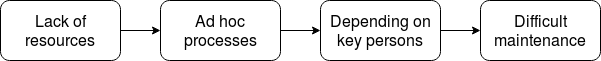
\includegraphics[width=0.9\textwidth]{images/Hasan2011-flow.png}
    \caption{Reason for challenges in software maintenance in small companies. Adapted from \citet[p.~5]{Hasan2011}}
    \label{fig:hasan-flow}
  \end{center}
\end{figure}

Many of the heavier maintenance processes also emphasize quality, which might not be the most important thing for rapidly growing small organizations \citep{Sanchez-Gordon2016}. This poses
a challenge on implementing standardized maintenance processes, since it would also require improving quality standards for example by refactoring. It has been shown that the main focus of
small companies is usually not in improving quality by refactoring as there rarely is enough resources for that \citep{Kajko-Mattsson2009}.
Therefore the small companies need more tailored
models of maintenance, some of which are proposed, but not extensively researched \citep{Hanssen2009}.

Another typical challenge for small companies is the lack of explicit portfolio management, which results in multitasking with different projects in parallel \citep{Vahaniitty2010}.
This encourages ad hoc processes and can be visible as "fire fighting" while trying to resolve issues with entirely different projects concurrently. Lack of strategic focus and
portfolio management could also lead to an overload of projects, which is not beneficial when considering quality and process aspects as the time pressure for ad hoc solutions
and poor maintainability grows. Additional effect of multitasking is assigning multiple roles for employees, meaning that 
the same employee could act as a business analyst, developer,
tester and sales representative at the same time, which reduces the productivity and efficiency of all processes that are operated in parallel \citep{Hasan2011}.

\section{Knowledge sharing in agile software development}
\label{section:knowledge-sharing}

There are mainly two types of knowledge: \emph{explicit} and \emph{tacit}. Explicit knowledge refers to knowledge that can be easily verbalized,
documented and shared with other individuals, whereas tacit knowledge is the exact opposite of that, meaning knowledge that can not be easily described
or shared via explicit documents \citep{Ryan2013}. Tacit knowledge is gained through
experience and learning by doing and it can not be learned from a book. In software development, sharing both is important, but tacit knowledge
has a much more significant effect on software development skills both on team and individual level and therefore sharing tacit knowledge
should be focused over explicit \citep{Ersoy2015}\citep{Ryan2013}.
This is especially important in agile software development as there is usually no explicit documentation available and development methods
rely on sharing tacit knowledge between team members \citep{Ryan2013}. Sharing tacit knowledge has also proven effects on performance and innovation
capabilities on team level \citep{Wang2012} and these effects are much more significant on smaller teams compared to larger ones as smaller teams tend
to work closer together \citep{Ersoy2015}.

In addition to performance improvements and encouraging innovation, sharing individual tacit knowledge to other team members reduces risks related to individuals
as there is always a possibility that they could have an accident, which forces them on a sick leave or they could just leave the company taking all of the acquired
tacit knowledge with them \citep{Ersoy2015}. The more tacit knowledge the person has, the more serious the risk becomes and therefore it should be addressed
accordingly. To reflect the phenomenon of shared knowledge and a "collective mind", \citet{Ryan2009} extend individual tacit knowledge to team level by introducing the concept of
team tacit knowledge, representing the knowledge that the group has. This is more than the sum of individual knowledge areas because individuals working as a team
can share and create new knowledge much easier and faster than the same individuals working alone.

The theoretical model for acquiring team level tacit knowledge by utilizing transactive memory system (TMS) is presented in figure \ref{fig:team-tacit},
which is originally presented by \citet{Ryan2013}. TMS was first defined by \citet{Wegner1987} as a shared storage of internal, external and transactive memories,
meaning that each individual in a group has access to certain information through the expertise of each other. The development of transactive memory is directly
related to the level of team tacit knowledge and therefore highly developed TMS improves team performance \citep{Ryan2013}.

\begin{figure}[ht]
  \begin{center}
    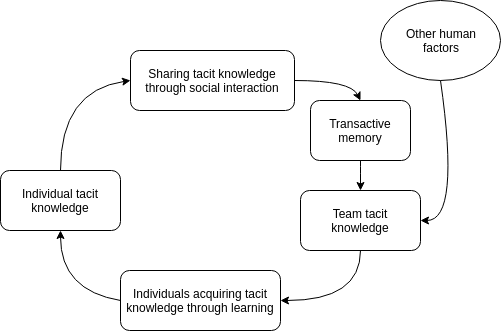
\includegraphics[width=0.9\textwidth]{images/Team-tacit-knowledge.png}
    \caption{Acquiring team tacit knowledge with transactive memory. Adapted from \citet[p.~8]{Ryan2013}}
    \label{fig:team-tacit}
  \end{center}
\end{figure}

The starting point for the acquisition cycle is the initial team tacit knowledge previously acquired by working together and sharing
experiences. This team level knowledge forms a base for individuals to construct their own thoughts and learn more, which then leads to a creation of individual tacit
knowledge. The most important part of the cycle is sharing tacit knowledge through social interaction and working together, which then eventually leads to an acquisition
of new team tacit knowledge through shared experiences. \citet{Ryan2013} emphasize the quality of social interaction as tacit knowledge is best shared in informal
face-to-face interactions between individuals. These interactions also help to develop the TMS for the team, which in turn leads to increased team tacit knowledge and
improved team performance. \citet{Ryan2013} also recognize that there are several other human factors in addition to social interactions and TMS that affect
the acquisition cycle. These factors include for example trust, leadership and team cohesion that also have a significant effect on team tacit knowledge creation
and the development of TMS and therefore they should not be neglected.

\subsection{Main challenges}
\label{section:barriers}

There are various challenges in knowledge sharing, some on general level and some specific to software development. \citet{Ersoy2015} group the challenges into three
main categories: \emph{sociological}, \emph{documentation} and \emph{implementation challenges}.

\subsubsection*{Sociological challenges}
The sociological challenges in knowledge sharing are related to human factors, not technical implementations or processes. One of the most significant sociological
challenges in knowledge sharing is the notion of knowledge as a property and the importance of its ownership. This is caused by considering
knowledge as power and rewarding individuals for having it, rather than sharing it, by higher salary for example. This encourages individuals to hoard
knowledge as they do not want to risk losing their position by sharing what they know. To prevent this, managers should start to recognize individuals for the
knowledge they share, not the knowledge they have and also give credit for knowledge products they create \citep{Dalkir2013}. This is the key to create a better
culture of knowledge sharing in an organization, which improves the performance and capability of the organization as a whole, but also requires
time to build.

Another sociological issue is the developer turnover rate as employees leaving the company will take the knowledge with them \citep{Ersoy2015}. There might be some
legacy projects that no one else has touched, which results in an orphaned code that no one is familiar with. This is especially problematic with strong code ownership
as individual employees become the key contributors in certain projects and do not want to share the ownership due to lack of trust for example \citep{Ersoy2015}.
Lack of trust can be present in both ways as those with the knowledge do not want to share it due to lack of trust on other persons, or those needing the knowledge
might not trust the knowledge provided due to lack of trust on expertise of the one with the knowledge \citep{Dalkir2013}. This is definitely a challenge of
organizational culture and needs to be taken seriously as it poses threats on team dynamics in general.
In addition to employees leaving the company, knowledge also tends to get forgotten over time if it is not actively used \citep{Basri2011}. This occurs frequently
and can not be entirely prevented, but sharing knowledge from individual level to the team level certainly helps to memorize the knowledge if it is needed again and thus reduces
knowledge loss.

Other considerations about sociological issues include practical issues such as working in different locations or during different times. This
decreases the amount and quality of social interactions which are essential in knowledge sharing. Additionally constant occupational stress reduces knowledge
sharing drastically. It could be caused by several different factors including organizational culture, team dynamics and workload for example. It
is important to notice the signs of stress as early as possible since it has a significant effect on knowledge sharing and team morale in general causing
lower performance and introducing new problems if not addressed properly. \citep{Ersoy2015}

\subsubsection*{Documentation challenges}

Documentation challenges in knowledge sharing are related to creating, using and maintaining explicit knowledge with documentation \citep{Ersoy2015}. Agile methodologies
generally do not emphasize extensive documentation and therefore documents used in agile development are generally informal, especially in the case of small companies
having less than 20 employees \citep{Basri2011}. However as \citet{Ersoy2015} argue, transferring explicit knowledge is difficult without proper documentation, which
is one of the reasons agile methodologies rely mostly on sharing tacit knowledge. \citet{Stettina2013} also argue that a formal handover between active development and
maintenance phases would help preventing knowledge loss, which also supports the argument of creating proper documentation. The need for documentation could be 
decreased by introducing the maintenance team to the project already during the active development phase, or even having the developers handle the maintenance phase as well.
However this does not remove the challenge of introducing new employees to the project either during the development or maintenance phase.

The most common issue with documentation after missing it entirely, is keeping relevant artifacts up to date \citep{Ersoy2015}\citep{Stettina2013}. This is problematic
as outdated information could lead to wasting time while working on already resolved issues or trying to get newer version of a project to work with outdated documentation.
Outdated documentation also lowers the value of updated documentation as developers might have concerns about the validity of it as well due to previous experiences of using
outdated documents.
This is one of the reasons agile methodologies emphasize the code itself as a documentation with clarifying comments if necessary \citep{Stettina2013}. By using the code itself 
as a documentation, it is guaranteed to be always up to date and usually properly version controlled, which ensures that the person is always looking at the documentation
that matches the executed code. Of course there is a risk that comments will be outdated after changes, which highlights the importance of readable code instead of relying
on clarifying comments. Another popular format for documentation is using a wiki, which could be beneficial for larger projects. However the practices should be carefully evaluated
as writing documentation for no one and without a purpose is a waste of resources and generally lowers the team morale \citep{Stettina2013}.

\subsubsection*{Implementation challenges}

Implementation challenges in knowledge sharing are related to the practical implementation of different knowledge sharing techniques and practices. One of the proposed
solutions to implement knowledge sharing in agile development is pair programming, which is further described in section \ref{section:pair-programming-theory}.
Pair programming has several benefits, most importantly encouraging knowledge sharing and improving the quality of the code being developed. However there are several practical issues
in implementing pair programming including pairing, lack of resources and motivation towards it. One of the reasons for lacking motivation for pair
programming is the skill level gap between the individuals participating on it. If, for example, junior team members are paired with the most senior ones, the seniors might
find less satisfaction in their job due to considering pair programming tasks simple and resource intensive. \citep{Ersoy2015} On the other hand, pairing junior team
members with each other does not encourage knowledge sharing as much as junior-senior pairs, which partly defeats the knowledge sharing purpose of pair
programming \citep{Sun2009}.
Additionally pair programming introduces scheduling issues as it requires more resources and increases the overall time consumed to complete the task at hand \citep{Ersoy2015}.

Another issue related to the practicalities of knowledge sharing is rapid pace of technological development \citep{Ersoy2015}. Rapid development of the technologies requires
more time spent while catching up with the latest trends and renders older knowledge outdated faster. Therefore the need for a constant effort to keep up with the
technologies could cause sociological issues such as stress and lack of trust on knowledge credibility, but also affect team dynamics as there might be differing opinions
about the latest development trends in used technologies.

\subsubsection*{Knowledge sharing barriers}

Literature sources generally refer to challenges in knowledge sharing as "barriers" since
their presence prevents effective knowledge sharing. There are several barriers suggested
in various sources and next the important barriers from software development point of view are listed and briefly explained. Recognizing these barriers helps to categorize
and solve knowledge sharing challenges as there are various studies describing the best practices to address each of them.

\emph{Lack of formal documentation} means missing official documents describing a software product or service. Formal documents are usually considered quite heavy and are
more common in large corporations rather than small agile organizations. Lacking proper formal documents could prevent knowledge sharing especially in larger
systems, depending on the context. \citep{Ghobadi2016}

\emph{Lack of informal documentation} means missing unofficial documents. In comparison to a formal documentation, informal documents can be of free format and varying
levels of quality. Informal documentation is more common in agile development as it is easier to create and maintain. If formal documents are missing or outdated,
informal documents should fill their purpose and lacking them therefore prevents efficient knowledge sharing. \citep{Ghobadi2016}

\emph{Lack of trust}, meaning lacking trust towards other employees and their knowledge. As already described in the previous sections, lack of trust is a significant issue in
knowledge sharing effectively preventing it totally and encouraging an unhealthy organizational culture. It is a serious issue and should be addressed with proper caution.
\citep{Ersoy2015}

\emph{Lack of comments in code}. As code itself generally acts as a documentation in agile methodologies, the importance of its clarity and quality increases. In some cases
the code can be further explained with additional comments and missing them in unclear parts of the codebase might lead to difficulties in knowledge sharing. \citep{Stettina2013}

\emph{Messy and complex code}. In addition to comments, the code itself acts as a documentation and it generally should be understandable without clarifying comments.
Having a messy and complex codebase becomes problematic over time as natural knowledge loss occurs and the codebase becomes legacy that no one knows in detail anymore.
Reducing complexity improves future maintainability and decreases the effect of forgetting unused knowledge over time. \citep{Stettina2013}

\emph{Lack of informal communication} is closely related to the acquisition cycle for tacit knowledge presented in figure \ref{fig:team-tacit}. As tacit knowledge is best shared through
informal social interactions, lacking them effectively breaks the cycle of acquiring team tacit knowledge eventually slowing the learning process of individuals as 
well. \citep{Ghobadi2016}

\emph{Knowledge hoarding} means refusing to share tacit knowledge with other persons due to its value or lack of trust. Hoarding is most likely a symptom of issues in 
the organizational culture and reward system as the reasons to hoard knowledge generally reflect the organizational dynamics. Therefore it can not be solved by forcing
individuals to share knowledge, but it needs to be addressed on an organizational level. \citep{Dalkir2013}

\emph{Difference in experience levels} could become an issue if it is so large that different persons do not generally have the same tools to discuss about specific
topics. This could cause frustration on more experienced employees when they need to explain the most simple concepts of some topic to less experienced colleagues, who on the
other hand will not benefit much from the discussion if they are lacking the basic knowledge on the subject and can not follow the explanation. This situation makes
knowledge sharing difficult and time consuming, which could affect other barriers by decreasing the amount of informal communication for example. \citep{Ghobadi2016}

\emph{Tight schedule} can prevent the usage of pair programming for example as it generally requires more time than solo programming. Tight schedules could also cause stress
and prevent knowledge sharing since there basically is no time available for knowledge sharing activities such as informal discussions. Tight scheduling might reflect
the problems on managerial side, which is why its root causes need to be identified for effective resolution. \citep{Ghobadi2016}

\emph{Lack of motivation} could also be a sign of managerial problems, but could also occur due to reasons completely outside of work environment. Either way, lack of
motivation towards working in general or knowledge sharing in particular affects the team dynamics negatively and could affect the motivation of team members as well.
It is important to identify the root cause for lacking motivation before it spreads further to the organization. \citep{Ghobadi2016}

\emph{Used communication tools} could be a preventive factor in knowledge sharing, especially if they are the main way of communication due to distributed locations for
example. One important factor is the usability of the communication tools as it greatly affects the quality of social interaction, but also the communication practices that 
are supported by those tools. It is important for the managers to analyze whether the tools actually support or prevent communication and to make changes if
considered necessary. \citep{Ghobadi2016}

\emph{Multitasking} means working on different projects or tasks in parallel so that one needs to constantly switch context from one to another. These context switches
decrease efficiency and quality of work as each time the context is switched, some time will be lost while readjusting the mindset to work on a new context. Time spent to
understand and solve the tasks is reduced and therefore learning and knowledge sharing is disturbed by constantly changing tasks, which could also increase stress.
\citep{Ghobadi2016}

\emph{Complex domain}, such as aviation industry, could also prevent knowledge sharing as its complexity requires much more
learning compared to simpler ones. It also effectively increases the knowledge
gap as novices will have to learn a lot to be even able to discuss with the experts using same terms. Complexity could also mean more tacit knowledge and make certain
aspects more difficult to verbalize so that they could be understood without a detailed knowledge about the related concepts. Working in a complex domain could also lead to 
knowledge hoarding as domain specific knowledge becomes an increasingly valuable asset when complexity increases. \citep{Ghobadi2016}

\emph{Working in different locations} naturally affects the communication between team members by reducing the amount of informal face-to-face interactions. Even though remote
working is popular in the software industry, it certainly affects the team dynamics and there should be clear rules about its practicalities to minimize the negative effects.
Special concern should also be on the used communication tools so that they will effectively support remote working and lower the barrier of knowledge sharing. \citep{Ghobadi2016}

\emph{Difference in age} is related to a gap in skill levels, but rather than being related to skills and terminology, it is more concerned about the social constructs during
interaction. The challenge is usually even more significant if a younger employee would be the expert and an older one the novice, which turns the social hierarchy upside down
and might be threatening or depressing to some persons. \citep{Riege2005}

\emph{Individual communication skills} are essential on daily discussions, both formal and informal, as weak communication skills generally lowers the quality of interactions
and could even lead to misunderstandings. Improvement of these skills is the responsibility of each person individually, but organization could help them to improve by
encouraging and giving constructive feedback. \citep{Riege2005}

\emph{Strong code ownership} is related to knowledge hoarding as individuals with strong ownership on a certain codebase are unwilling to share their knowledge and ownership
of it. This can become an issue if these individuals leave the company or are otherwise unavailable to answer the questions about the codebase. There is no shared knowledge about the
codebase and gathering it without the key persons might be difficult. In the worst cases, the project becomes legacy and requires heavy re-engineering before any
further updates can be made to it. \citep{Riege2005}

\emph{Physical work environment} can also prevent knowledge sharing, since if the workspace does not support team activities or informal discussions, the amount and quality
of interactions will decrease. This is an important aspect to keep in mind while considering changes at the office. Managers could support knowledge sharing by providing
enough group working rooms with sufficient equipment such as screens and whiteboards to support co-working. \citep{Riege2005}

\emph{Organizational culture} is one of the key aspects in knowledge sharing since if it does not support and encourage knowledge sharing, there will be significant performance
and team working issues. Organizational culture itself is hard to measure and define, but there are plenty of other barriers that could be present due to issues in
organizational culture, which makes it an influential aspect that should be considered and evaluated frequently. \citep{Riege2005}

\emph{Strong organizational structure} or hierarchy could also prevent organization wide knowledge sharing and encourage individual work. If there are for example
strict rules about communication between different teams, the amount of interactions between the teams most likely decreases.
Also if the organization relies too heavily on top-down management, there will not be knowledge co-creation on team level,
which could improve performance and innovation capabilities. \citep{Riege2005}

\section{Software process improvement}

Processes are a crucial part of software development and their efficiency can make a difference between success and failure. It has also been recognized that software process
improvement (SPI) is one of the key challenges for small and medium sized software companies and therefore it should be taken seriously \citep{Sulayman2009}.
According to the lean ideology the processes should be under continuous improvement, which makes them similar to agile software development with small incremental
iterations to react to changing requirements. \citet{Osterweil2011} argues that software processes can be treated exactly the same
as software itself and therefore SPI can be addressed with similar methodologies as software development, including iterations and continuous improvements.

There are various frameworks to implement these improvements, most notably Capability Maturity Model Integration (CMMI),
which is used to evaluate the maturity of a software organization. CMMI includes 22 processes to measure and improve, which can be evaluated either with four capability levels
in a continuous representation (\emph{incomplete}, \emph{performed}, \emph{managed} and \emph{defined}) or with five maturity levels in a staged representation (\emph{initial}, \emph{managed},
\emph{defined}, \emph{quantitatively managed} and \emph{optimizing}) \citep{CMMIProductTeam2010}. This maturity model can be used to evaluate internal processes or a subcontractor for example.
However, it is not exactly suitable for small organizations since small organizations in general do not have the resources required to implement full SPI programs that are more targeted towards
large corporations \citep{Mishra2009b}. There has been an identified need for tailored SPI frameworks for small organizations and several have also been suggested, one of them being \emph{an Approach
for Software Process Establishment in Micro and Small Companies} (ASPE-MSC) model that is especially tailored to meet the requirements of these companies \citep{Mishra2009b}. It is based on
various other approaches consisting of three main phases: \emph{planning}, \emph{monitoring and control} and \emph{post-mortem}. The planning phase includes also the implementation itself whereas
monitoring and control acts as a rapid feedback for the effectiveness of the plan and suggests updates if necessary. The post-mortem phase then focuses on gathering feedback about the iteration to
prepare for the next one. The whole process is facilitated by a process engineer, that is usually suggested to be an external consultant to achieve the best results.

Generally the most challenging part of SPI or any other process improvement is lack of motivation and commitment towards it, both from senior management and employees \citep{Allison2010}.
Therefore to succeed in process improvement, a key factor is senior management commitment that significantly reflects to motivation of other personnel as well. However, the managerial commitment alone is
not enough as the improvement will be implemented by the employees after all, which makes involvement and influence to their daily activities a major focus point. \citep{Herranz2014}
The main difference between large and small companies on SPI is the level of commitment, which is usually high in small companies \citep{Basri2010a}. Therefore the key challenge
of SPI in small organizations is not commitment to change, but lack of resources, which is especially problematic when considering implementing SPI frameworks. As budget and deadlines
are already tight, there is rarely extra personnel available to facilitate SPI, even though it could yield a high return of investment in the future \citep{Allison2010}\citep{Larrucea2016}.
Additionally processes in small organizations are generally informal and small, which makes applying standardized SPI frameworks useless \citep{Basri2010a}. In addition, despite the high
commitment on process improvement, there might be change resistance also present in small organizations as people generally would like to stick to the habits they are used to, rather than
experimenting with new ones \citep{Larrucea2016}. This could be a result of prior experiences on failed process improvement experiments and therefore it is important to address these
experiences before implementing any improvements to avoid facing issues related to them \citep{Allison2010}.

Despite various challenges and a possibility of a failure in SPI, it has several benefits that make it worth the effort. In addition to improved performance and efficiency, improved processes
can also lead to an increased customer satisfaction due to faster delivery times and a better customer service. Improved processes also tend to yield more satisfied development
teams as they can focus on completing their work efficiently rather than wasting time on inefficient processes, which can mean for example having unprepared meetings with a wide audience.
This naturally increases productivity as well. \citep{Sulayman2009} On the other hand also the company culture can be improved by SPI as having efficient processes and high job satisfaction
correlates with more flexible and open organizational culture. \citet{Lee2016} also argue that a clan-like culture, where the whole organization is like a family with low hierarchy, supports
knowledge sharing much better than the traditional hierarchical culture. As a conclusion, it can be argued that SPI greatly supports organizational development on various aspects in addition to
improved business performance.

\section{Measuring software maintenance}
\label{section:literature-metrics}

To succeed in SPI, it is important to be able to measure the initial state and changes in it. There are various metrics proposed to measure different aspects of
software maintenance. The most relevant ones for this case context are briefly listed below and they are later evaluated together with custom defined metrics in section
\ref{section:measuring}.

\emph{Reopen rate} - The ratio of reopened tickets basically meaning that the tickets have been marked as resolved, but the resolution did not satisfy the original reporter
and thus they need to be readdressed. A high reopen rate could indicate a need for further technical training for the maintenance personnel or deeper problems with projects in
general. \citep{Livy2017}

\emph{Tickets resolved on the first iteration} - The ratio of tickets resolved on the first try without a need for further communication. A higher rate usually correlates with
better customer satisfaction and the overall maturity of the maintenance personnel. \citep{Livy2017}

\emph{SLA violations} - The ratio of service level agreement (SLA) violations out of all tickets. Higher ratio indicates severe problems in maintenance process as the company fails to meet
its SLA compliance, which is most likely a violation of maintenance contract. A higher ratio could indicate lack of resources on the maintenance process, but could also
mean that the maintenance personnel are unaware of the SLA limits. Either way, this is an important metric for the business side of the maintenance process. \citep{Livy2017}

\emph{Cost of a ticket} - Internal cost of solving incidents. This metric helps to identify the most expensive tickets so that their resolution process can be improved.
This is one of the important aspects to measure when evaluating the business performance of the maintenance process. \citep{Livy2017}

\emph{Response time} - Time between reporting and the first reaction to a ticket. Could correlate with customer satisfaction as faster response times usually mean
more satisfied customers. A longer average response time could also indicate lack of resources and correlate with several other metrics such as resolution times and the number of
active tickets. \citep{Paschke2006}

\emph{Resolution time} - The average time to resolve tickets on each level. This fits together with the SLA violation ratio and it can provide early warnings when
the resolution times are growing so that changes can be made before the SLA limits are violated. This metric works as a good measurement on the overall performance of the
maintenance process and could also correlate with customer satisfaction. Therefore it could be argued that it is a good general metric for the maintenance process. \citep{Livy2017}

\emph{Customer satisfaction} - Not a well-defined metric like others, but still an important aspect to measure on the maintenance process. Customer satisfaction could be
correlated with other metrics such as resolution time and reopen rate, but it would still be beneficial to define a direct way to measure satisfaction itself. \citep{Livy2017}

\emph{Number of active tickets} - The amount of tickets that have been reported, but are not yet resolved. An increasing number of concurrently active tickets could mean
lack of resources on the maintenance process as the personnel can not resolve the tickets fast enough to keep up with the pace of newly created tickets. This could correlate with
reopen rate and is most likely also visible as longer resolution times, but it is good to have it as a separate metric to identify lack of resources early enough
before things get worse. \citep{Livy2017}

\emph{Tickets by criticality} - The amount of tickets on each criticality level. For example a higher amount of high priority issues could indicate issues in the latest releases and
therefore quality assurance, but could also mean vaguely defined criticality criteria, which could be a sign of immaturity of the maintenance process. \citep{Livy2017}

\emph{Tickets from unofficial sources} - The amount or ratio of tickets reported outside of the official maintenance process. This metric is only an approximation of all unofficial
tickets since not all of them will ever be visible in the official maintenance process, but it still gives an approximation of the problem. A higher amount of unofficial tickets
could indicate problems in the customer interface of the main process or just lack of training on the customer side. Either way it would be good to direct more of the unofficial
tickets to the official process. \citep{Livy2017}

\emph{Ticket count per project or team} - The tickets grouped by projects or teams. This metric could help indicate problematic projects or teams that require a more detailed
inspection of the root causes for problems \citep{Livy2017}. Could be beneficial, but could also lower team morale if not addressed in a considerate way.

\emph{System downtime} - A direct measurement on availability of the system. This could be included in the maintenance contract making it an important measure. Tolerance for
downtime naturally depends highly on the context and the business criticality of the system. \citep{Paschke2006}

\section{Common solutions}
\label{section:solutions-theory}

As the challenges of software maintenance and knowledge sharing presented in the previous sections are quite well studied, there are also several proposed solutions intended to solve them.
The most suitable solutions for the context of this case study are presented here and together they represent a good variety of different solutions that could be applied to solve the
challenges of the case company.

\subsection{Pair programming}
\label{section:pair-programming-theory}

As sharing tacit knowledge is generally hard and requires effort, it is often considered a challenge in software companies. One excellent method for knowledge
sharing and especially transferring tacit knowledge is pair programming. It generally means that two persons are working together on one computer so that one is doing the task, being the
\emph{driver}, while the other one is constantly observing, being the \emph{navigator} \citep{Williams2010}\citep{Wray2010}. They are constantly discussing about the task at hand, evaluating different aspects
of the problem and creating the solution together. The roles are not fixed and they can be constantly changed on the fly whenever necessary to achieve the best results \citep{Gupta2013}\citep{Wray2010}.

Although it has not been universally proven to be always beneficial \citep{Maguire2014}, there are several claimed benefits of pair programming that can occur if organized successfully.
First of all, pair programming encourages sharing especially tacit knowledge between individuals \citep{Maguire2014}\citep{Plonka2015}\citep{Williams2010}\citep{Wray2010}\citep{Zieris2014}. By working on 
the same task on one computer, individuals automatically start to communicate about the task and share thoughts about the solution, which leads to a mutual understanding and knowledge
co-creation while solving the task at hand. Knowledge sharing effect works the best with pairs of one junior and one senior when junior is acting as the \emph{driver} actually conducting the
task and senior is acting as the \emph{navigator} by giving advice and mentoring the junior to solve the task \citep{Plonka2012}\citep{Plonka2015}\citep{Sun2009}. This forces the senior to verbalize
knowledge instead of just working with the task while the junior is trying to keep up with the pace and eventually disengages from the task \citep{Plonka2012}\citep{Plonka2015}.

In addition to knowledge sharing, literature also suggests that pair programming could help to solve problems faster \citep{Hannay2009}\citep{Lui2010}\citep{Wray2010}, improve code quality
\citep{Hannay2009}\citep{Williams2010}\citep{Wray2010} and improve team spirit \citep{Maguire2014}\citep{Stapel2010}\citep{Williams2010}. First of all, it has been shown that the overall resolution
time for tasks of any complexity could be faster than solving the task individually \citep{Hannay2009}\citep{Lui2010}\citep{Sun2009}. However this comes with a cost of investing the time
of two persons rather than just one, which results in a higher cost for solving the task \citep{Lui2010}\citep{Spohrer2013}\citep{Williams2010}. Secondly, improved quality of code is evident as there are constantly
two persons who can spot mistakes easier \citep{Spohrer2013}\citep{Wray2010} and push for working according to the best practices \citep{Williams2010}\citep{Wray2010}. The effect of pair pressure also
causes both persons to concentrate on the task at hand rather than switching to private tasks frequently \citep{Sillitti2011}\citep{Stapel2010}\citep{Williams2010}\citep{Wray2010}. However it has been
shown that while gaining more experience and being more familiar with each other, the amount of off-topic discussions is likely to increase \citep{Stapel2010}. Off-topic discussions are not inherently
a bad thing as they help to increase team spirit and might ease out conversations about the actual topic as well \citep{Williams2010}. These off-topic discussions could be directed towards breaks between
tasks by agreeing about common guidelines on pair programming \citep{Maguire2014} and having a physical work environment that supports both concentration and informal discussions \citep{Mishra2009a}.

However these benefits do not come without a cost. The main drawback of pair programming is the increased investment of human capital especially with people without prior experience of
pair programming \citep{Spohrer2013}\citep{Williams2010}. Due to this, pair programming is not the best approach for situations with a high market pressure or tight scheduling since solo programming
is more efficient when considering the total cost of solving the task \citep{Sun2009}. Another key challenge to address is disengagement, meaning that the one acting as a navigator can be tempted
to lose focus on the task at hand due to time pressure or being unable to follow the driver's work \citep{Plonka2012}\citep{Williams2010}. This could be solved by letting the junior act as a driver and carefully selecting
the tasks to be solved with pair programming \citep{Plonka2012}. In addition to selecting the tasks, it is also important to select the right pairs to solve them
\citep{Gupta2013}\citep{Hannay2009}\citep{Sun2009}\citep{Williams2010}. As mentioned, junior-senior pairs generally result in the best knowledge sharing experience,
but sometimes the task requires the highest possible quality, meaning that
senior-senior pair would be a better choice \citep{Sun2009}. It is also important to rotate the pairs frequently so that the employees get experiences with different partners and their working habits \citep{Spohrer2013}\citep{Williams2010}.

\subsection{README}
\label{section:readme-theory}

Since agile methodologies do not generally encourage creating and maintaining an extensive documentation \citep{Basri2011}\citep{Gupta2013},
but lacking proper documents is still a major challenge in knowledge sharing \citep{Ersoy2015}, some compromise between heavy documentation and lacking one entirely is needed.
One proposed solution to create and maintain lighter, more informal documentation is a "README" file. It is usually located in the root directory of a project's codebase and written in a plaintext
format, such as markdown \citep{Karimzadeh2016}\citep{VanGompel2016}. It is especially important in open source community as it gives the first impression to anyone visiting the
codebase and acts as a summary of the project \citep{Karimzadeh2016}\citep{Prana2018}. There is no single standardized structure for a README and there are various practices that
are highly context dependent, although generally the README aims to provide answers to "what" and "how" questions about the project \citep{Prana2018}.

The most common contents of the README include some background or a high-level description of the project, usage examples and building and installation instructions
\citep{Ikeda2019}\citep{Karimzadeh2016}\citep{Prana2018}\citep{VanGompel2016}. In addition to those, also updated support information, environments, release notes and links to further documentation
could be included, but these are naturally dependent on the context of the project \citep{Ikeda2019}\citep{Karimzadeh2016}\citep{VanGompel2016}. \citet{Ikeda2019} also point out that
some form of a task list or known limitations alongside with the application programming interface (API) documentation could be added to the README if considered necessary. The clear benefit of
including these details alongside the codebase is the fact that documentation tends to get outdated quite rapidly and having it in version control system together with the codebase
encourages updating it more frequently and usually results in a better updated documentation, even though it would be in an informal format \citep{VanGompel2016}. Informal documents such as
README files also act as a support for project handover and ensure that critical knowledge is kept together with the codebase to avoid knowledge loss \citep{Stettina2013}.

\subsection{Project presentations}
\label{section:presentations-theory}

Another solution to tackle knowledge sharing challenges and improve available informal documentation, could be regular presentations about different ongoing projects. Presentation as
a communication method is probably familiar to most people already from school since they are commonly used in education, but also regularly in a work environment \citep{Bhattacharyya2011}.
Therefore most people should be quite familiar about giving presentations about different subjects under their expertise. A clear benefit of giving presentations is also the fact
that it forces the experts to share their knowledge in a concise and structured format, which might clarify the topic for themselves as well. Also since it is beneficial to have
a slide show to support learning \citep{Wecker2012}, informal and concise documentation is created as a side effect.

The natural drawback of the presentations is the effort that is required to prepare them in contrast to the expected benefits. It can be also seen as an additional work that prevents
working on actual tasks that are considered more important, which could cause lack of motivation towards presentations. Additionally the applicability of a slide show as documentation could
be debatable and it could get outdated quite fast, which could lead to misconceptions in the worst case.

\subsection{Triaging}
\label{section:triage-theory}

The initial incidents reported to the ticket tracking system could be of varying quality. Some might be very detailed with precise descriptions, while others do not provide enough
information to even start working on the ticket. This is challenging as it could be time consuming to actually identify what the ticket is about and who could solve it.
The problem effectively gets worse while the amount of tickets grows and therefore a structured approach, such as a triaging process, is needed.
In software context triage means gathering
all the necessary information needed to solve the ticket, before finding the right person to assign it to \citep{Ruefle2013}. This way developers can focus on
development tasks rather than having to deal with vaguely defined incidents that might be entirely out of their area of expertise. With low ticket volumes this process can be done
manually, but once the company grows and a growing amount of tickets floods the help desk, the manual techniques do not scale very well and the maintenance personnel will eventually be unable to handle new tickets
\citep{Hu2014}. This is why various automatic processes for triaging incidents are proposed. These are usually based on machine learning techniques with hundreds of thousands of
sample incidents as a training material and their purpose is usually to evaluate the priority and find the right assignee for the incident \citep{Hu2014}. Because of the need for training data,
these techniques are mainly suitable for large corporations or open source communities with a large amount of historical incidents recorded in the database.

Improving ticket quality is beneficial for all stakeholders participating in the maintenance process as an issue tracking system should be the main medium for communication between
them, containing all the information related to the ticket handling process \citep{Bertram2010}. However, customer might not have the technical expertise to report incidents with all
the details required to efficiently solve them and on the other hand, developers most likely do not have time and motivation to constantly check for newly created tickets when 
there is also some new development to be done. A solution to this problem of shared responsibility would be job rotation \citep{Faegri2009}
and a rotating triage responsibility. This way the developers could focus on their main tasks while spending some predetermined time to triage tickets for other developers.
This could be an efficient solution, but its implementation needs to be carefully considered as people still like to get their main tasks done efficiently and adding additional
job rotation to slow down the main activities could cause loss of motivation \citep{Faegri2009}.

\subsection{Automatic alerts}
\label{section:alerts-theory}

Another way to improve ticket quality is to detect the incidents automatically, before anyone needs to report them manually. This can be done with improved application
monitoring, which alerts the maintenance personnel if certain conditions are met.
There are various aspects that cloud application monitoring could benefit, troubleshooting being only one of them
\citep{Aceto2013}, but as cloud application management is a relatively new concept in the field due to an increased popularity of cloud services, their efficient management is still
quite challenging and heavily context dependent \citep{Fatema2014}. One of the most challenging tasks is to find the right set of key performance indicators (KPI) to measure.
This is especially important in SaaS business as the amount of customers could be constantly growing and an automatic detection of incidents and performance issues significantly improves
the service quality \citep{Shao2010}.

The most significant benefit of automatic alerts in comparison to customer created tickets is the quality and amount of details included. As alerts are generated automatically
on predefined events, it is much easier to find the root cause of the incident and make more informed decisions about its priority for example \citep{Aceto2013}\citep{Fatema2014}\citep{Shao2010}.
These alerts should be connected to the help desk in order to add them to the maintenance process rather than directly notifying individual
developers or even teams \citep{Hernantes2015}. The main challenge with alerts is recognizing the need for alert in different situations as they are highly context dependent
and it might be easy to create a lot of unnecessary alerts about performance issues that do not require any actual actions to be taken. On the other hand failing to alert about
actual incidents is also a problem and therefore the right balance between unnecessary and missing alerts should be determined based on the business criticality of the system.

\subsection{Transition model}
\label{section:transition-theory}

An important phase in software lifecycle management is the transition from active development to maintenance mode. During this transition there is a risk for losing information
due to lack of updated documentation delivered for the maintenance personnel, which results in inefficient maintenance \citep{Stettina2013}. One of the most important factors for
any project is the background information about its context, business case and requirements and this information is lost easily as it is rarely documented anywhere while using
agile development methodologies \citep{Ito2016}. One solution to this problem is introducing maintenance personnel to the project already during development, or even having
developers also do the maintenance work \citep{Stettina2013}. This however does not solve the risk of personnel changes during maintenance by an employee leaving the company or
new employees joining to the team \citep{Ito2016} and therefore it is important to have an actual transition model from active development to maintenance, including standardized
requirements for documentation and maintenance practicalities.

\citet{Ito2016} identify three main challenges for transition. These are unrevised documents, unclear background knowledge and omitting necessary information. They suggest that
the challenge of having unrevised documentation out of sync with the actual codebase could be solved by adding an update history to each document clarifying the latest changes to them.
\citet{Stettina2013} also highlight developers' mindset of creating documentation for someone else and thus lacking the motivation for adding detailed information. Commitment to
artifacts is generally a challenge alongside with a time pressure leading to lower quality documentation lacking the necessary information \citep{Stettina2013}. This could be tackled
by encouraging informal documents like README files (see section \ref{section:readme-theory}) and storing them with the codebase to encourage updates to them. Additionally documentation
files should be reviewed by other team members or maintenance personnel, and updated based on their feedback about the necessary information \citep{Ito2016}.

\subsection{WIP limits}
\label{section:wip-theory}

As time pressure and multitasking are a major problem for knowledge sharing, tackling them should be taken seriously. One way to manage time pressure and parallel streams
of work in agile development is WIP limits. Their main purpose is to ensure that the previous tickets have been finished before new ones can be started, which could prevent over commitment
that easily leads to time pressure and multitasking \citep{Ahmad2016}. If implemented correctly, WIP limits could improve the efficiency of both maintenance and development processes \citep{Concas2013}.
However, introducing limits most likely does not solve the root cause of the problems, but it encourages tackling them as multitasking is no longer an option. Also introducing new strict
practices to daily activities is not an easy task as it requires commitment from the whole team \citep{Ahmad2013} and a clear internal prioritization of different tasks, which might be
problematic in some contexts.
